% \cleardoublepage

\newrefsection

\chapter{外文翻译: 扩散偏好标注:直接偏好判断高效对齐LLM}

论文标题:Spread Preference Annotation: Direct Preference JUDGMENT FOR EFFICIENT LLM ALIGNMENT

作者:Dongyoung Kim、Kimin Lee、Jinwoo Shin等

\sectionnonum{摘要}

对齐大型语言模型(LLMs)以符合人类偏好已成为实现最先进性能的关键步骤,然而,构建大规模的人类标注偏好数据集的成本极高。
为了解决这一问题,我们提出了一种新的框架——扩散偏好标注 (Spread Preference Annotation, SPA),
该框架通过直接偏好判断来提升 LLM 的对齐能力,仅需极少量的人类标注偏好数据。我们的核心思想是利用小规模(种子)数据中的人类先验知识,并通过迭代生成响应和从自标注偏好数据中学习,不断提高 LLM 的对齐效果。
具体而言,我们提出从 LLM 的 logits 中推导偏好标签,以显式提取模型的内在偏好。
相比于使用外部奖励模型或隐式上下文学习的现有方法,我们观察到该方法明显更为有效。
此外,我们引入了一种噪声感知偏好学习算法,以缓解生成偏好数据中潜在低质量信息的影响。
实验结果表明,该框架能够显著提升 LLM 的对齐性能。
例如,在 Ultrafeedback 数据中仅使用 3.3\% 的真实偏好标签,我们在 AlpacaEval 2.0 评测中达到了比使用全部数据或最先进基线方法更优的对齐效果。

\section{介绍}

近年来,大型语言模型(LLMs)在各种自然语言处理(NLP)任务上取得了巨大进展,
推动了代码助手和聊天机器人等被数百万用户使用的现实世界应用 \citep{claude3, openai2022chatgpt, team2023gemini}。  
使 LLMs 与人类反馈对齐,尤其是通过学习人类偏好,
被广泛认为是其成功的关键技术 \citep{christiano2017deep, lee2021pebble, ziegler2019fine}。  
为增强这种对齐,各种偏好学习算法被广泛研究 \citep{ouyang2022training, rafailov2023direct}。  
尽管取得了诸多进展,但当前仍面临的一个挑战是对大规模人类标注偏好数据的依赖。  
由于偏好数据的质量和数量对 LLMs 的成功对齐至关重要 \citep{bai2022training, cui2023ultrafeedback},获取这些数据的巨大成本无疑构成了重大障碍。  

为缓解这一挑战,让 LLMs 参与构建偏好数据并利用这些数据提升对齐能力的研究最近受到了关注。  
例如,一种典型的方法是针对输入提示生成多个响应,并通过 LLM 预测来近似人类偏好,
这通常被称为\textit{LLM 作为评判者(LLM-as-judge)} \citep{bai2022constitutional, yuan2024self}。  
然而,这些方法仅在 LLM 足够大且对齐良好时,才能有效地通过上下文学习模拟人类偏好。  
另一方面,使用外部奖励模型来高效替代人类偏好标注是一个可行方案 \citep{jiang2023llm, snorkel2024pairrm},
但这种方法依赖于大量人类偏好数据,并且如果数据分布不匹配,也可能失效。  
此外,这些方法可能会受到 LLM 生成的潜在标注噪声的影响,而这一方面尚未得到充分研究。  
因此,在本研究中,我们的目标是提出一种方法,以克服上述限制,并在仅依赖少量人类标注的情况下,有效提高 LLM 的对齐能力。  

\begin{figure*}[t]
    \centering
    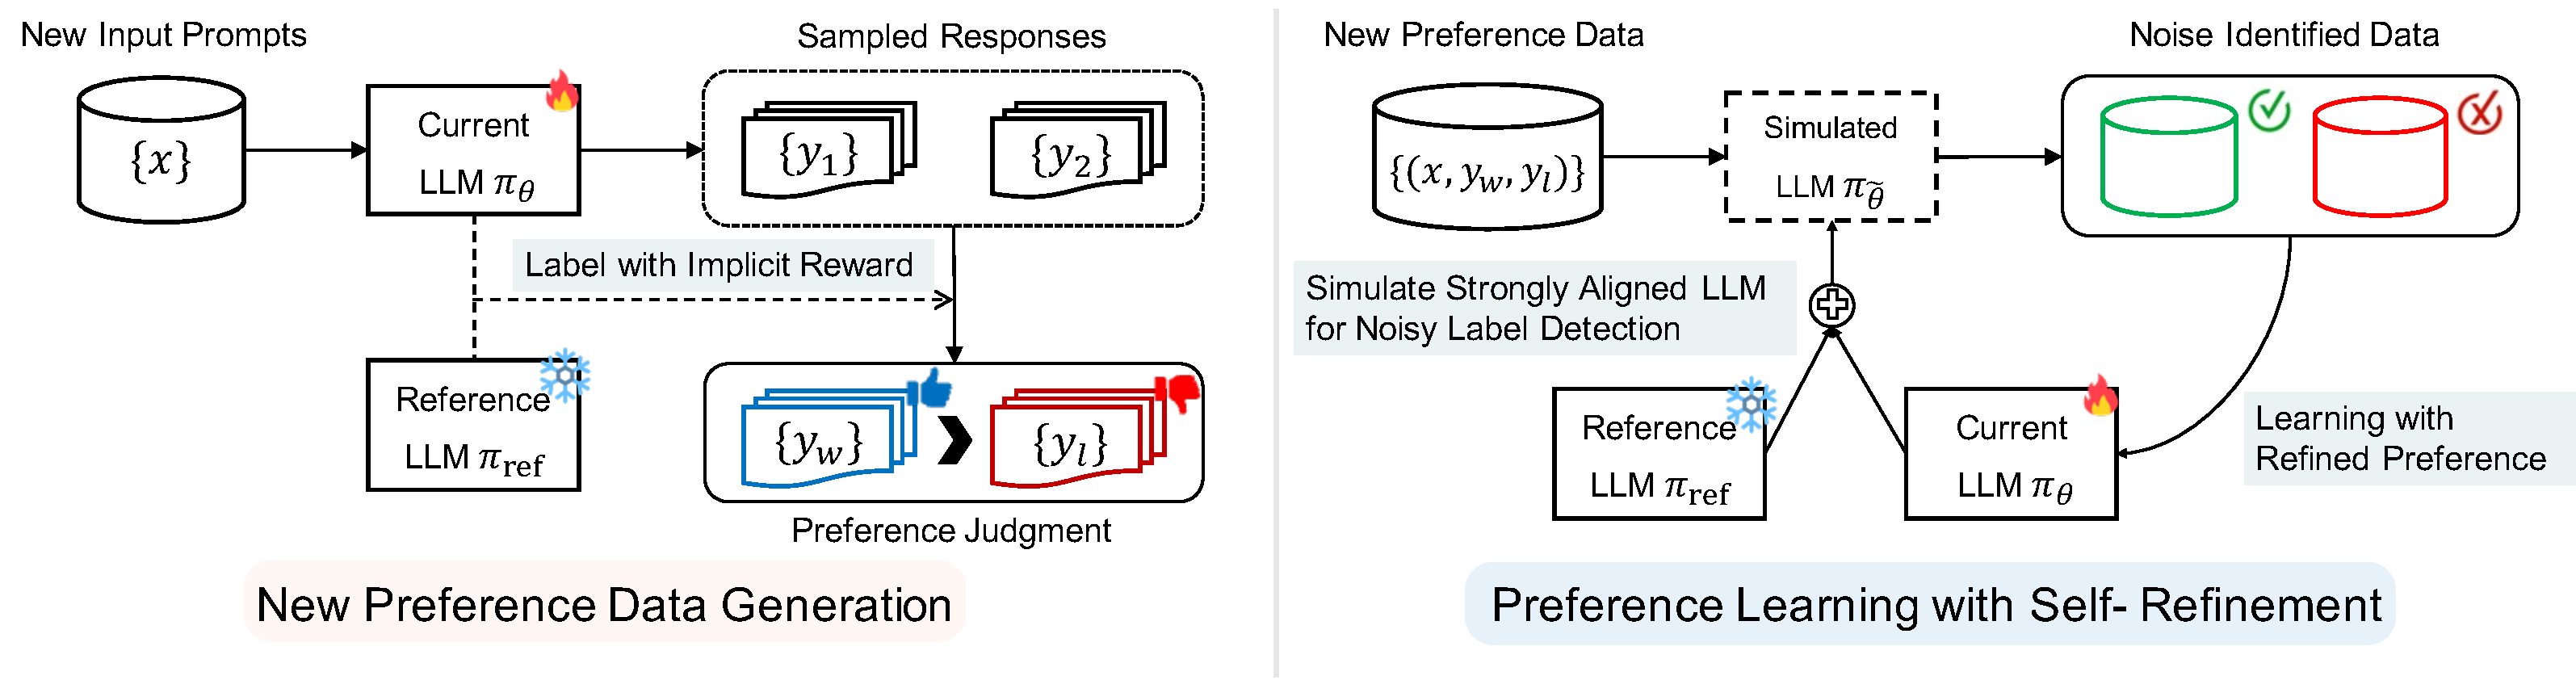
\includegraphics[width=1.0\textwidth]{figure/raw_files/main.pdf}
    \caption{\textbf{所提出的 SPA 框架的示意图。} SPA 通过迭代 (1) 生成新的偏好数据 和 (2) 在构造的数据上进行带有自我优化的偏好学习,逐步提高 LLM 的对齐程度。}
    \label{fig:illustration}
    \vspace{-0.1in}
\end{figure*}

\textbf{贡献:}  
我们提出了一个简单但有效的框架,称为 SPA,通过\textbf{S}preading \textbf{P}reference \textbf{A}nnotation\textbf{, SPA)}的方式,
仅依赖少量人类标注的偏好数据,利用\textbf{直接偏好判断}来提升 LLM 的对齐能力。  
我们的核心思想是在小规模(种子)数据的基础上,\textbf{逐步扩展}人类偏好知识,
\textbf{通过迭代生成响应并利用自标注的偏好标签进行学习},从而提升 LLM 的对齐效果。  

具体而言,我们的技术贡献包括以下三个方面:  

1. \textbf{直接从 LLM 的 logits 评判偏好标签},以显式提取模型的内在偏好。这一方法比依赖外部奖励模型或隐式上下文学习的现有方法更为有效。

2. \textbf{引入基于置信度的偏好标签优化},以降低生成数据中偏好学习的噪声风险。

3. \textbf{提出线性外推预测方法},在当前模型与参考模型之间进行预测外推,以模拟更强对齐的模型预测,从而\textbf{提高噪声识别能力},进一步增强偏好标签优化的效果。

\begin{figure}[t]
    \centering
	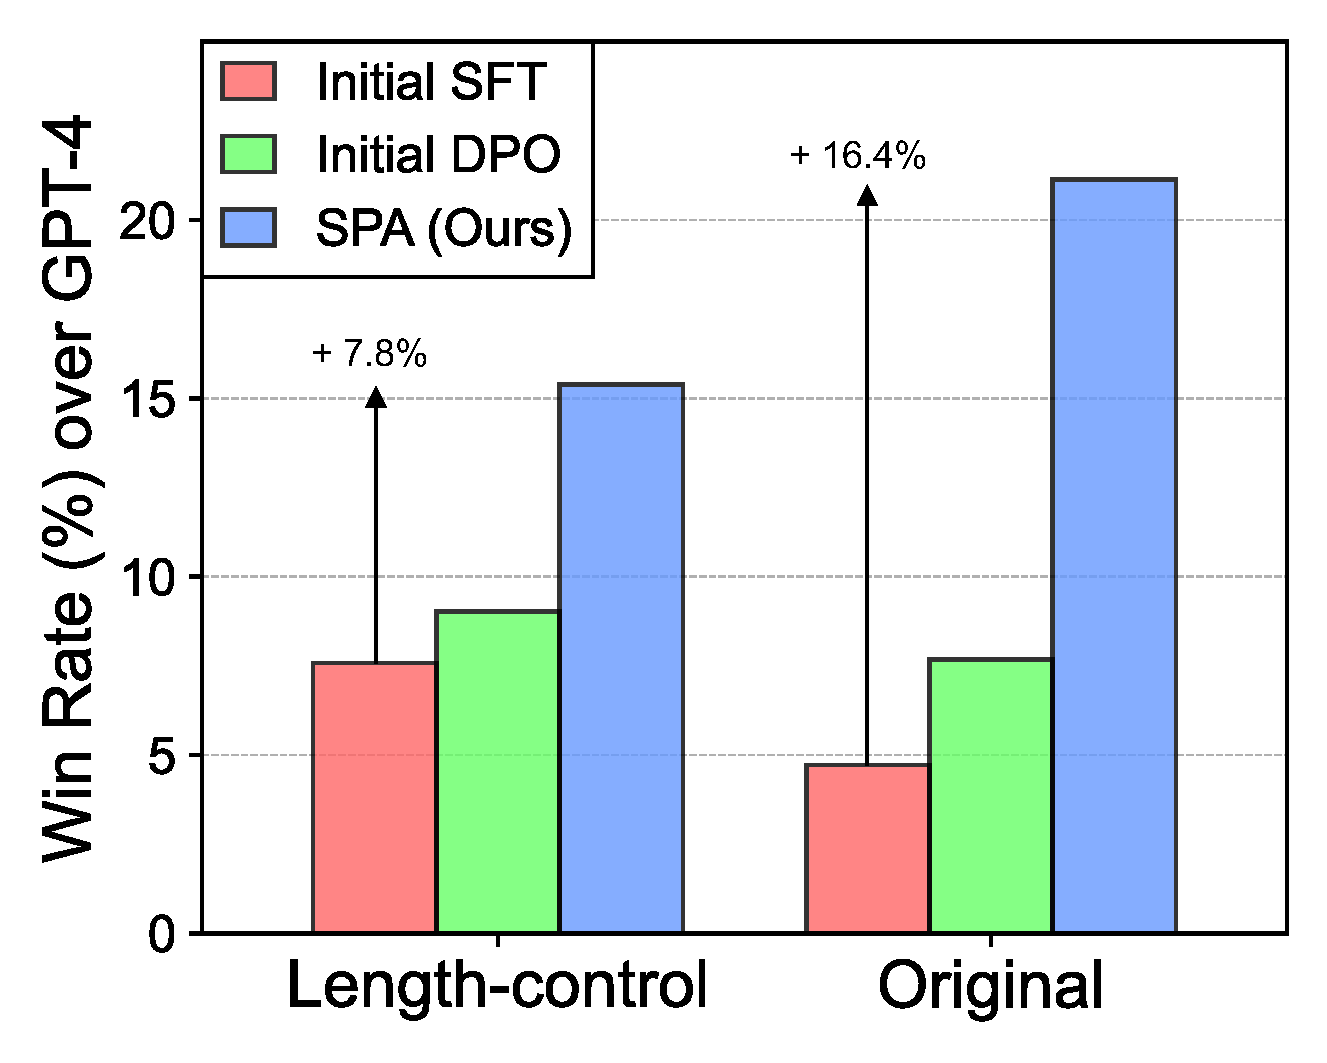
\includegraphics[width=50mm]{figure/raw_files/iclr25_spa_fig2.pdf}
	\vspace{-0.5cm}
    \caption{\textbf{主要结果总结。} 在 AlpacaEval 2.0 \citep{alpaca_eval} 上的评估结果。我们的框架在没有额外人类偏好数据的情况下显著提升了 LLM 的对齐程度。}
    \label{fig:summary}
\end{figure}

我们通过使用少量人工标注的偏好数据对最新的 LLM 进行对齐,并在常用基准上评估其对齐程度,从而证明了所提出的 SPA 的有效性。  
例如,在 Ultrafeedback 数据 \citep{cui2023ultrafeedback} 中仅使用 3.3\% 的真实偏好数据,
并基于 mistral-7b-0.1v SFT 模型 \citep{jiang2023mistral} 进行实验,
我们的框架在 AlpacaEval 2.0 \citep{alpaca_eval} 上的胜率相比初始 SFT 模型提升了 16.4\% 以上(见图 \ref{fig:summary})。  
此外,AlpacaEval 2.0 的长度控制胜率从 7.58\% 提高至 15.39\%,MT-bench 分数 \citep{zheng2023judging} 从 6.38 提升至 6.94。  
与 LLM-as-judge \citep{zheng2023judging} 等偏好判断方法相比,
甚至与最近在 AlpacaEval 2.0 基准上表现最优的强奖励模型 PairRM \citep{jiang2023llm} 相比,我们的方法在所有指标上均取得了更优的表现。  
更有趣的是,所提出的 SPA 即使在没有初始人类偏好数据的情况下,也能成功提升各种 LLM 的对齐程度。  
这些结果表明,我们的框架在实际应用中极具竞争力和实用性。  

\section{相关工作}
\textbf{LLM 与人类偏好的对齐。}
从人类偏好中学习已成为最新 LLM 的核心组成部分 \citep{claude3, openai2023gpt4, team2023gemini, touvron2023llama},
用于使其响应更符合用户的意图和价值观 \citep{ouyang2022training, ziegler2019fine}。  
可以说,最流行的框架之一是基于人类偏好的强化学习(RLHF)\citep{christiano2017deep, lee2021pebble},
其首先训练奖励模型,然后通过 KL 散度正则化微调 LLM 以最大化该奖励,从而防止 LLM 的奖励过度优化。  
另一方面,近年来提出了多种偏好学习算法,以更高效地利用人类偏好微调 LLM 
\citep{ethayarajh2024kto, hong2024orpo, liu2023statistical, rafailov2023direct, xu2023some, zhao2023slic, meng2024simpo}。 
例如,\citet{rafailov2023direct} 提出了直接偏好优化(DPO),其通过数学推导得出与 RLHF 等价的训练目标,从而无需单独训练奖励模型即可微调 LLM。 
\citet{ethayarajh2024kto} 进一步消除了对成对偏好标签的依赖,基于人类效用模型构建训练目标。 
然而,这些方法都假设可用大量人工标注的偏好数据,而这通常需要巨大的数据获取成本。 

\textbf{利用 LLM 构建偏好数据。}  
为了实现高效且可扩展的对齐过程,近年来利用 LLM 进行偏好数据集构建受到关注。  
一种常见的方法是让 LLM 生成多个对同一输入提示的响应,并利用 LLM 的预测来近似人类对这些响应的偏好,这种技术通常被称为 \textit{LLM-as-judge} \citep{bai2022training, yuan2024self}。  
然而,只有当 LLM 规模足够大且对齐良好时,该方法才能通过上下文学习有效地模拟人类偏好。  
另一种方法是使用外部奖励模型来替代人类偏好判断 \citep{jiang2023llm, snorkel2024pairrm},该方法可以更高效地进行偏好估计,但依赖于大量人类偏好数据来预训练奖励模型,并且在数据分布不匹配的情况下可能效果不佳。  
一些最新研究 \citep{rosset2024direct, snorkel2024pairrm, wu2024self, xiong2024iterative} 提出了结合迭代数据扩展与偏好学习的对齐方法,  
但它们通常依赖外部奖励模型或更强大的 LLM 进行偏好判断。  
相比之下,我们仅利用训练中的 LLM 内在知识来进行新数据扩展和偏好学习。  
\cite{chen2025bootstrapping} 同时提出了一个类似的想法,重点关注长度正则化,而我们的工作则专注于通过所提出的自我优化过程提升生成数据的质量。  

\section{预备内容}\label{sec:preliminary}

设 LLM 为 $\pi_{\theta}$,其针对给定的输入序列(\textit{e.g.}, 提示词)$x$ 生成输出序列(\textit{e.g.}, 响应)$y$,
即 $y \sim \pi_{\theta}(\cdot|x)$。  
我们的目标是使 $\pi_{\theta}$ 对各种输入提示提供符合人类偏好的响应。  
为此,我们采用广泛使用的偏好学习框架,该框架通过优化 $\pi_{\theta}$ 以学习人类对两个不同响应的偏好 
\citep{christiano2017deep,lee2021pebble,ouyang2022training}。  
具体而言,我们假设偏好数据集 $\mathcal{D}=\{(x,y_l,y_w)\}$ 可用,其中包含输入提示 $x$、偏好响应 $y_w$ 以及非偏好响应 $y_l$ 的三元组。  
这里,偏好标签由真实标注者(通常是人类专家)进行标注。  

\textbf{奖励建模与强化学习微调。}  
由于难以直接对 $y_w$ 和 $y_l$ 之间的成对偏好进行建模,常见的方法是引入奖励函数 $r(x,y)$,
并基于 Bradley-Terry 模型 \citep{bradley1952rank} 对偏好进行建模:
\begin{equation}
p(y_{w} \succ y_{l} \mid x) = \frac{\exp\left(r(x, y_w)\right)}{\exp\left(r(x, y_w)\right) + \exp\left(r(x, y_l)\right)}.
\label{eq:bt_reward}
\end{equation}

根据该公式,可以通过最大似然目标函数对参数化的奖励模型 $r_{\phi}(x,y)$ 进行估计:
\begin{equation}
    \mathcal{L}_R(r_\phi) = -\mathbb{E}_{(x, y_w, y_l) \sim \mathcal{D}} \left[ \log \sigma \left( r_\phi(x, y_w) - r_\phi(x, y_l) \right) \right].
\end{equation}

其中,$\sigma$ 为 sigmoid 函数。  
在完成奖励建模后,可以通过优化 LLM $\pi_{\theta}$ 以最大化 $r_\phi$ 所捕获的奖励,从而提升其对齐程度。  
通常,KL 散度正则项被引入,以防止 $\pi_{\theta}$ 过度优化奖励,
该正则项相对于参考模型 $\pi_{\text{ref}}$ 计算,
并受超参数 $\beta > 0$ 控制 \citep{ouyang2022training, ziegler2019fine}:
\footnote{$\pi_{\text{ref}}$ 通常由监督微调(SFT)LLM 初始化 \citep{chung2024scaling, wei2022finetuned},
同时 $\pi_{\theta}$ 也初始化为 $\pi_{\text{ref}}$。}  
\begin{equation}
\mathcal{L}_\text{RLHF}(\pi_{\theta}) = -\mathbb{E}_{y \sim \pi_{\theta}, x \sim \rho} \left[ r_{\phi}(x,y) \right] + \beta \mathrm{D}_{\mathrm{KL}} \left( \pi_{\theta}(y|x) \parallel \pi_{\text{ref}}(y|x) \right).
\label{eq:rlhf}
\end{equation}

\textbf{直接偏好建模与优化。}  
\citet{rafailov2023direct} 提出了一种将 LLM $\pi_{\theta}$ 与偏好数据集 $\mathcal{D}$ 进行对齐的替代方法,称为直接偏好优化(DPO)。
DPO 将奖励建模和强化学习微调这两个对齐步骤整合为一个统一的微调过程。
具体而言,最优奖励函数可从 RLHF 目标(方程 \ref{eq:rlhf})推导出来,
并基于目标 LLM $\pi_{\theta}$ 以及参考模型 $\pi_{\text{ref}}$ 
\citep{go2023aligning, peng2019advantage, peters2007reinforcement}:
\begin{equation}\label{eq:orig_reward}
r(x, y) = \beta \log \frac{\pi_{\theta}(y \mid x)}{\pi_{\text{ref}}(y \mid x)} + \beta \log Z(x),~\text{where}~Z(x) = \sum_y \pi_{\text{ref}}(y \mid x) \exp \left( \frac{1}{\beta} r(x, y) \right). 
\end{equation}

随后,可以使用该奖励函数来衡量两个响应之间的偏好,并优化 $\pi_{\theta}$ 以最大化偏好数据集 $\mathcal{D}$ 中 $y_w$ 相对于 $y_l$ 的偏好:
\begin{equation}\label{eq:orig_pref}
    p_{\theta}(y_{w} \succ y_{l} | x) = \sigma \left(\beta \log \frac{\pi_{\theta}(y_w|x)}{\pi_{\text{ref}}(y_w|x)} - \beta \log \frac{\pi_{\theta}(y_l|x)}{\pi_{\text{ref}}(y_l|x)}\right).
\end{equation}
\begin{equation}\label{eq:dpo_objective}
    \mathcal{L}_\text{DPO}(\pi_{\theta}) = \mathbb{E}_{(x, y_w, y_l) \sim \mathcal{D}} \left[-\log p_{\theta}(y_{w} \succ y_{l} | x) \right].
\end{equation}

\section{SPA:扩展偏好标注以提升 LLM 对齐性} \label{sec:method}

\textbf{概述。}
在本节中,我们介绍 SPA:\textbf{S}pread \textbf{P}reference \textbf{A}nnotation 通过直接偏好判断来对齐 LLM,同时降低构建偏好数据集的巨大成本。  
我们的核心思想是充分利用小规模(种子)数据中的人类先验知识,并逐步更新 LLM 以提升对齐性。  
具体来说,SPA 迭代执行两个步骤:(1)通过自生成偏好进行数据扩展(第 \ref{sec:method:data_expansion} 节)和(2)
通过自优化偏好学习对 LLM 进行微调(第 \ref{sec:method:self_refine} 节)。  
整体流程请参考图 \ref{fig:illustration}。  

\textbf{初始阶段:}  
我们假设给定了一个小规模(种子)偏好数据集 $D_0$ 和一个初始 LLM $\pi_{\text{init}}$。  
这里,我们遵循常见的做法 \citep{ouyang2022training, rafailov2023direct, ziegler2019fine},
使用已经在指令数据集上经过监督微调(SFT)的 LLM 作为 $\pi_{\text{init}}$ \citep{chung2024scaling, wei2022finetuned},但它尚未与人类偏好对齐。
然后,我们首先通过在数据集 \(D_0\) 上使用 DPO \citep{rafailov2023direct}(方程 \ref{eq:dpo_objective})对 \(\pi_{\text{init}}\) 进行微调,从而获得弱对齐的大模型 \(\pi_0\)。  
在众多偏好学习方法中,我们选择 DPO,是因为它具有简单性和有效性。

\subsection{通过自生成数据进行直接偏好判断来对齐 LLMs}\label{sec:method:data_expansion}

对于第 $i$ 次迭代($i=1, \dots$),我们假设新的提示集 $X_{i}=\{x\}$ 已经可用,即 $X_{i} \cap X_{j} = \emptyset$ 对所有 $j=0, \dots, i-1$.\footnote{$X_{0}=\{x|(x,y_l,y_w) \in \mathcal{D}_{0}$\}} 
从 $X_{i}$ 中,我们通过使用 LLM 的内在生成和奖励建模能力构建第 $i$ 次人工偏好数据集 $\mathcal{D}_{i}=\{(x,y_l,y_w)|x \in X_{i}\}$。
具体来说,对于每个输入提示 $x \in X_{i}$,我们从 $\pi_{i-1}$ 中采样两个响应 $y_1$ 和 $y_2$,即 $y_1, y_2 \sim \pi_{i-1}(x)$,其中 $\pi_{i-1}$ 是上一次迭代的结果模型。
然后,利用通过 $\pi_{i-1}$ 和 $\pi_{\text{init}}$(方程 \ref{eq:orig_reward})捕获的奖励,我们测量 $\pi_{i-1}$ 在 $y_1$ 和 $y_2$ 之间的偏好:

\begin{equation}\label{eq:our_pref}
    p_{i-1}(y_{1} \succ y_{2} | x) = \sigma \left(\beta \log \frac{\pi_{i-1}(y_1|x)}{\pi_{\text{init}}(y_1|x)} - \beta \log \frac{\pi_{i-1}(y_2|x)}{\pi_{\text{init}}(y_2|x)}\right).
\end{equation}

然后,我们根据以下方式直接判断偏好标签,并通过此方式构建 $\mathcal{D}_{i}$:
\begin{equation}\label{eq:our_label}
    (y_{w}, y_{l}) = (y_{1}, y_{2})~\text{ 如果 }~p_{i-1}(y_{1} \succ y_{2} | x) > 0.5~\text{ 否则 }~(y_{w}, y_{l}) = (y_{2}, y_{1}).
\end{equation}

\begin{algorithm}[t!]
    \caption{SPA 算法}
    \label{alg:main}
 \begin{algorithmic}
   \STATE
   \textbf{输入:} 初始模型 $\pi_{\text{init}}$,种子偏好数据集 $\mathcal{D}_{0}$,迭代次数 $T$,新提示集 $\{X_{i}\}_{i=1}^{T}$,  
   \vspace{0.05in} 
   \hrule
   \vspace{0.05in}  
   \STATE 使用 DPO 训练 $\pi_{\text{init}}$ 和 $\mathcal{D}_{0}$(方程 \ref{eq:dpo_objective}),获取初始弱对齐模型 $\pi_{0}$  
   \FOR{$t=1$ {\bfseries 到} $T$}
   \STATE 通过 $\pi_{t-1}$ 和 ${X}_{t}$ 合成偏好数据 $\mathcal{D}_{t}$(方程 \ref{eq:our_pref} 和 \ref{eq:our_label})
   \STATE 初始化训练模型和参考模型 $\pi_{\theta} \leftarrow \pi_{t-1}$, $\pi_{\text{ref}} \leftarrow \pi_{t-1}$  
   \FOR{小批量样本 $B \sim \mathcal{D}_{t}$}
   \STATE $z_{\widetilde{\theta}} \leftarrow \text{对 } B \text{ 进行去耦噪声检测,基于 } \pi_{\theta}, \pi_{\text{ref}}, {X}_{t}$(方程 \ref{eq:noise_realign} 和 \ref{eq:detail_realign})
   \STATE 计算训练损失 $\mathcal{L}_{\text{rf}}$,基于 $z_{\widetilde{\theta}}$ 和 $\pi_{\theta}$ 进行偏好标签优化(方程 \ref{eq:self_refine_combined})
   \STATE 更新模型参数: $\theta \leftarrow \theta - \eta  \nabla_{\theta}\mathcal{L}_{\text{rf}}$
   \ENDFOR
   \STATE 初始化下一次迭代模型 $\pi_{t}$,使用更新后的参数 $\theta$
   \ENDFOR
   \STATE \textbf{返回}~~$\pi_{T}$
 \end{algorithmic}
\end{algorithm}

\subsection{生成偏好数据的自优化以实现高效学习} \label{sec:method:self_refine}  
在构建 $\mathcal{D}_i$ 之后,我们通过微调 $\pi_{\theta}$ 进行第 $i$ 轮偏好学习,
其中 $\pi_{\theta}$ 由 $\pi_{i-1}$ 初始化,并使用 DPO 进行训练(此处,我们还将 $\pi_{i-1}$ 作为方程 \ref{eq:dpo_objective} 中的 $\pi_{\text{ref}}$)。  
学习自生成的偏好数据 $\mathcal{D}_i$ 可以利用 LLM 的能力有效地传播 $\mathcal{D}_0$ 中的人类偏好先验,从而提高对齐性。  
然而,这一过程也可能受到潜在标签噪声的影响,该噪声可能源于 $X_i$ 的分布偏移或 $\pi_{i-1}$ 在奖励建模方面的不足。  
因此,我们进一步提出了一种改进的偏好学习方法,利用一种新颖的去噪技术:\textit{通过\textbf{解耦噪声检测}进行偏好标签的\textbf{自优化}}。  

\textbf{偏好标签的自优化}:  
我们的核心直觉是,推导出的偏好(方程 \ref{eq:orig_pref})可以被视为当前训练中的 LLM $\pi_{\theta}$ 对 $\pi_{i-1}$ 分配标签的置信度。  
当给定的响应对较难判别时,$\pi_{\theta}$ 可能表现出较低的置信度,表明存在较高的标签噪声概率。  
值得注意的是,置信度在噪声标签学习领域中是最常见的衡量指标之一 \citep{han2018co, reed2014training, sohn2020fixmatch}。  
基于这一直觉,我们首先识别置信度最低的 $K$\% 样本:
\begin{equation}\label{eq:naive_noise_detection}
    z_{\theta}=1~ 
    \text{ 如果 }~p_{\theta}(y_{w} \succ y_{l} | x)<\tau~\text{ 否则 }~z_{\theta}=0,
\end{equation}
其中,$\tau$ 是数据集 $\mathcal{D}_i$ 中置信度排名第 $K$ 百分位的样本的置信度。  
然后,利用该(潜在的)噪声识别标签 $z_\theta$,我们采用标签平滑 \citep{muller2019does} 来优化偏好标签,
以便在高噪声风险(\textit{即},$z_{\theta}=1$)的情况下减少 $\pi_{\theta}$ 的训练置信度:
\begin{equation} \label{eq:self_refine_combined}
    \mathcal{L}_\text{rf}(\pi_{\theta}) = \mathbb{E}_{(x, y_w, y_l) \sim \mathcal{D}_i} \left[-\big((1-\alpha \ast z_{\theta}) \log p_{\theta}(y_{w} \succ y_{l} | x) + \alpha \ast z_{\theta} \log p_{\theta}(y_{l} \succ y_{w} | x) \big)\right], 
\end{equation}
其中,$\alpha$ 是超参数。  
然后,我们使用 $\mathcal{L}_\text{rf}(\pi_{\theta})$ 来训练 $\pi_{\theta}$,以替代原始的 DPO 训练目标(方程 \ref{eq:dpo_objective})。  

\textbf{解耦噪声偏好检测}:  
虽然使用优化后的偏好标签可以降低 $\pi_{\theta}$ 学习噪声偏好的风险,但由于用于噪声检测的模型 $\pi_{\theta}$ 来源于标签生成模型 $\pi_{i-1}$,其有效性可能受到限制。  
因此,为了进一步提升偏好标签优化框架的有效性,我们引入了解耦噪声检测(de-coupled noise detection)\citep{han2018co, li2020dividemix} 技术以对齐 LLM。  
具体而言,我们通过模仿一个更强对齐的 LLM $\pi_{\widetilde{\theta}}$ 的偏好预测来识别偏好噪声:
\footnote{在方程 \ref{eq:detail_realign} 中的 $\lambda$ 设定下,$\pi_{\widetilde{\theta}}$ 相当于通过方程 \ref{eq:rlhf} 训练得到的模型,其 KL 项比 $\pi_{\theta}$ 小 $(1 + \lambda)$ 倍。}
\begin{equation}\label{eq:noise_realign}
    z_{\widetilde{\theta}}=1~ 
    \text{ 如果 }~p_{\widetilde{\theta}}(y_{w} \succ y_{l} | x)<\tau~\text{ 否则 }~z_{\widetilde{\theta}}=0.
\end{equation}

借助这种解耦标识方式,我们在方程 \ref{eq:self_refine_combined} 的基础上使用优化的偏好标签训练 $\pi_{\theta}$,\textit{即},用 $z_{\widetilde{\theta}}$ 替换方程 \ref{eq:self_refine_combined} 中的 $z_{\theta}$。  
这里,我们通过 $\pi_{\theta}$ 和 $\pi_{\text{ref}}$ 的 logit 线性组合来近似计算 $\pi_{\widetilde{\theta}}$ 的 logit $h_{\widetilde{\theta}}$:
\footnote{当 $\pi_{\theta}(\cdot|x):=\text{Softmax}\big(h_{\theta}(x)\big)$ 时,我们将 $h_{\theta}(x)$ 视为 LLM $\pi_{\theta}$ 在给定输入 $x$ 下的 logit。}  
这种方法受到最近研究的启发 \citep{liu2024decoding},该研究表明,不同 $\beta$ 值的 RLHF 对齐模型是参考模型和单一对齐模型的几何混合:
\begin{equation}\label{eq:detail_realign}
    h_{\widetilde{\theta}}(x,y_{1:t-1})  = (1 + \lambda) \ast h_{\theta}(x, y_{1:t-1}) - \lambda \ast h_{\text{ref}}(x, y_{1:t-1}),
\end{equation}

其中,$\lambda > 0$ 是超参数,$y_{1:t-1}$ 表示在第 $t$ 个输出之前的输出序列。  

值得注意的是,这种通过近似 $p_{\widetilde{\theta}}(y_{w} \succ y_{l} | x)$ 进行的解耦噪声检测\textit{不会增加额外计算开销},因为所需的 $h_{\theta}$ 和 $h_{\text{ref}}$ 在计算原始 DPO 目标(方程 \ref{eq:dpo_objective})时已经获得。  
因此,SPA 仅需在原始 DPO 代码基础上添加少量额外代码即可实现。  
我们在算法 \ref{alg:main} 中展示了 SPA 的完整流程。

\section{实验} \label{sec:experiments}

在本节中,我们展示实验结果,以回答以下问题:
\begin{itemize}[leftmargin=5.5mm,topsep=0pt]\vspace{-0.04in}
    \item[$\circ$] SPA 是否仅利用少量人工标注的偏好数据即可提高 LLM 的对齐能力?(表~\ref{tab:main_result},图 \ref{fig:res_no_seed})\vspace{-0.04in}
    \item[$\circ$] 我们提出的方法是否优于其他偏好标注方法?(表~\ref{tab:judgments},图 \ref{fig:res_iteration})\vspace{-0.04in}
    \item[$\circ$] SPA 是否在不同种类的种子数据和 LLM 设定下都具有泛化能力?(表~\ref{tab:diff_N_seeds},\ref{tab:variance_seeds},\ref{tab:phi})\vspace{-0.04in}
    \item[$\circ$] SPA 中的各个组件对最终效果的影响是什么?(表~\ref{tab:ablation},\ref{tab:add_analyses})\vspace{-0.04in}
\end{itemize}

\subsection{实验设置} \label{sec:5.1}

\textbf{模型.}  
若未作特殊说明,我们的实验均使用经过监督微调的 Mistral-7b-0.1 模型 \citep{jiang2023mistral} 作为初始模型 $\pi_{\text{init}}$(参见第 \ref{sec:method} 节)。  
具体而言,我们使用了开源模型\footnote{\url{alignment-handbook/zephyr-7b-sft-full}},该模型遵循 Zephyr \citep{tunstall2023zephyr} 训练策略,并在 Ultrachat \citep{ding2023enhancing} 指令数据上进行了微调。  
更多细节见附录。

\textbf{基线方法.}  
为了评估所提出的偏好判断方法(方程 \ref{eq:our_pref})的有效性,我们与其他偏好判断方法进行了比较。  
具体而言,我们考虑了使用迭代 DPO(Iterative DPO)\citep{snorkel2024pairrm, xu2023some} 训练模型的基线方法,该方法通过 LLM 作为评判者(LLM-as-judge)\citep{bai2022constitutional, zheng2023judging}(即上下文学习)或外部强大奖励模型(如 PairRM \citep{jiang2023llm})来生成偏好数据并更新模型。  
值得注意的是,这些方法在去除 SPA 的自我优化(self-refinement)组件后,与 SPA 仅在评判方法上有所不同。  
详细内容见附录。

\textbf{数据集.}  
在偏好学习任务中,我们使用 UltraFeedback 数据集 \citep{cui2023ultrafeedback},与之前的研究保持一致 \citep{snorkel2024pairrm, rosset2024direct}。\footnote{\url{"argilla/ultrafeedback-binarized-preferences-cleaned"}}  
具体而言,我们首先从该数据集中构建种子数据,包含 2K 个样本(占 60K 数据的 3.3\%),每个样本包含提示(prompt)、模型生成的回复(response)和人工标注的真实偏好标签。  
在表 \ref{tab:main_result} 和 \ref{tab:phi} 中,我们将 UltraFeedback 提供的真实偏好标签称为\textit{金标准标签}(gold label)。  
然后,我们将剩余的数据划分为 8K、20K 和 30K 三个子集,仅保留提示部分。  
这些子集分别用于迭代阶段 1、2 和 3 的提示集。  
仅在表 \ref{tab:diff_N_seeds} 的实验中,我们改变了种子数据的大小。  

\textbf{评估方法.}  
遵循 LLM 对齐的常见实践,我们主要采用以下两种评测方法来评估每个模型的表现:  
(1) AlpacaEval 2.0 \citep{dubois2023alpacafarm, dubois2024length, alpaca_eval}。  
AlpacaEval 2.0 旨在近似评估模型在指令跟随任务中的人类偏好。  
该评测使用来自多个数据集的 805 条指令,并通过比较 GPT-4 \citep{openai2023gpt4} 与测试模型的响应来计算胜率(win rate)。  
为了缓解 LLM 偏好的长度偏差问题 \citep{wang2023far, zheng2023judging},我们同时测量原始胜率和长度控制(LC)胜率。  
其中,LC 胜率是通过一个单独训练的回归模型 \citep{dubois2024length} 对响应长度影响进行中和后的调整胜率,以便更专注于质量评估。  
(2) 我们还使用 MT-Bench \citep{zheng2023judging} 评估 LLM 的多方面能力。  
具体来说,MT-Bench 评测聊天机器人在多个类别(如数学、编程、角色扮演、写作等)上的综合能力。  
评测通过 GPT-4 对多轮对话问题的回答进行评分。  
这些基准测试可全面评估 LLM 在对齐人类偏好方面的表现及其实际应用中的整体有效性。  

\textbf{实现细节.}  
在初始化阶段之后,我们进行三轮数据扩展,每轮使用模型自生成的偏好数据。  
在数据扩展过程中,我们针对每个提示(prompt)独立采样 2 个响应,采样温度设为 0.7。  
然后,使用 SFT 模型作为参考模型,我们根据方程 \ref{eq:our_pref} 进行偏好标注。  
为了获得初始模型 $\pi_0$,我们在种子数据集上进行了 3 轮 DPO 训练。  
在随后的每次迭代训练中,仅进行 1 轮训练。  
DPO 训练的超参数 $\beta$ 设定为固定值 $\beta = 0.1$。  
批量大小设为 32,学习率为 $5 \times 10^{-7}$。  
我们采用 AdamW 优化器,并使用余弦学习率调度器,其中 10\% 的训练步骤作为预热阶段。  
对于 SPA 的超参数 $\alpha$ 和 $K\%$,我们使用固定值 $\alpha = 0.1$ 和 $K = 10$。  
此外,在去噪阶段,我们加入了预热机制,使去噪在完成 20\% 训练步骤后才被激活。  
在去耦合噪声检测的超参数 $\lambda$ 设定上,我们在迭代 1、2 和 3 轮中分别使用逐步递减的值 1/2、1/4 和 1/8。  

\begin{table}[t]
    \centering
    \caption{\textbf{主要结果。} 在 AlpacaEval 2.0 和 MT-Bench 上,不同 Mistral-7B-v0.1 变体的评估结果。最佳分数以 \textbf{加粗} 标出。}
    \begin{tabular}{lc|cc|c}
    \toprule
     & & \multicolumn{2}{c|}{\textbf{AlpacaEval 2.0}} & \textbf{MT-Bench} \\
    \cmidrule(lr){3-4} \cmidrule(lr){5-5}
    Models & \begin{tabular}{@{}c@{}} Gold \\ Label (\%)\end{tabular}& \begin{tabular}{@{}c@{}}Len-control. \\ Win Rate (\%)\end{tabular} & \begin{tabular}{@{}c@{}}Win Rate \\ vs. GPT-4 (\%)\end{tabular} & \begin{tabular}{@{}c@{}}Avg. Score \\ (0-10) \end{tabular} \\ \midrule
    Mistral-7B-v0.1 & - & 0.17 & 0.50  & 3.25 \\
    Zephyr-7b-$\beta$ & 100 & 11.75 & 10.03 & 6.87 \\\midrule
    SFT & - & 7.58 & 4.72 & 6.34 \\ 
    DPO & 3.3 & 9.03 & 7.68 & 6.81  \\ 
    SPA (Ours) & 3.3 & \textbf{15.39} & \textbf{21.13} & \textbf{6.94} \\
    \bottomrule
    \end{tabular}
    \label{tab:main_result}
\end{table}

\begin{table}[t]
    \centering
    \caption{\textbf{偏好判断基线比较。} 在 AlpacaEval 2.0 和 MT-Bench 上,使用不同偏好判断方法对迭代训练模型(从 SFT 模型开始)进行评估的结果。最佳分数以 \textbf{加粗} 标出。}% \begin{adjustbox}{width=0.9\linewidth}
    \resizebox{\textwidth}{!}{
    \begin{tabular}{lc|cc|c}
    \toprule 
     & & \multicolumn{2}{c|}{\textbf{AlpacaEval 2.0}} & \textbf{MT-Bench} \\
    \cmidrule(lr){3-4} \cmidrule(lr){5-5}
    Methods & \begin{tabular}{@{}c@{}} External \\ Model  \end{tabular} & \begin{tabular}{@{}c@{}}Len-control. \\ Win Rate (\%)\end{tabular} & \begin{tabular}{@{}c@{}}Win Rate \\ vs. GPT-4 (\%)\end{tabular} & \begin{tabular}{@{}c@{}} Avg. Score \\ (0-10)  \end{tabular}  \\ \midrule
    Iterative DPO (PairRM) & O & 11.87  & 9.46 & \textbf{6.98}  \\
    Iterative DPO (LLM-as-judge) & X & 9.28  & 9.18 & 6.67  \\
    SPA (Ours) & X & \textbf{15.39}  & \textbf{21.13} & 6.94 \\ \bottomrule
    \end{tabular}
    }
    % \end{adjustbox}
    \label{tab:judgments}
\end{table}

\subsection{主要结果}\label{sec:5.2}
在完成 3 轮数据扩展和通过 SPA 进行微调后,训练得到的模型在 AlpacaEval 2.0 基准测试中的对 GPT-4 的胜率达到了 21.13\%,如表 \ref{tab:main_result} 所示。
相比于仅使用 3.3\% 的标注数据并采用标准 DPO 训练时的 7.68\% 胜率(7.68\% $\rightarrow$ 21.13\%),这一结果表明了显著的提升,同时长度控制胜率也有所提升(9.03\% $\rightarrow$ 15.39\%)。
此外,SPA 在 MT-Bench 上获得了 6.94 的分数,明显优于使用相同 3.3\% 标注数据进行 DPO 训练的模型(6.81)。
更有趣的是,我们的方法在胜率(10.03\% vs 21.13\%)和长度控制胜率(11.75\% vs 15.39\%)方面均优于 Zephyr-7b-$\beta$,后者使用了相同的基础模型(Mistral-7B-0.1v)和 SFT 数据集,但采用了显著更多的标注偏好数据,即 UltraFeedback 数据集的 100\%(相比之下 SPA 仅使用 3.3\%)。
在胜率上的这些显著提升清楚地表明了 SPA 所带来的整体性能增强。

接下来,在表 \ref{tab:judgments} 中,我们提供了额外的实验结果,以验证所提出的偏好判断方法。具体而言,表 \ref{tab:judgments} 中的三个实验可以被视为采用不同偏好判断方法的迭代 DPO 变体。从中可以观察到,SPA 相较于其他方法表现显著更优。具体来说,SPA 在 AlpacaEval 2.0 基准上对抗 GPT-4 的胜率达到 21.13\%,相比之下,使用外部奖励模型 PairRM 作为基线的胜率仅为 9.46\%。在长度控制胜率方面,SPA 也取得了 15.39\% 的成绩,超越了奖励模型的 11.84\%。 

我们推测,使用训练中的 LLM 进行直接偏好判断的迭代 DPO 训练方法能够优于从外部奖励模型推断标签的情况,其主要原因与分布偏移(distribution shift)有关。随着迭代次数的增加,LLM 生成的数据分布会逐渐偏离种子偏好数据的分布。此时,外部奖励模型的有效性不可避免地下降,因为奖励模型是固定的,而生成的数据却越来越远离其训练分布。相比之下,SPA 通过不断更新的内在奖励模型生成偏好标签,因此在迭代过程中受到分布偏移的影响较小,从而在迭代训练中表现更为有效。

关于这一点,我们在图 \ref{fig:res_iteration} 中的实验结果也提供了支持。在第 1 轮迭代中,两种方法的有效性相差不大。然而,在第 2 轮迭代时,性能差距显著拉大,这一结果从实验上支持了上述推论。

另一方面,使用上下文学习(in-context learning)方法的 LLM 作为判断器(LLM-as-judge)在胜率方面与 PairRM 相当,但在长度控制胜率方面表现较差(11.87\% vs 9.28\%),这表明 LLM-as-judge 方法存在局限性。总体而言,实验结果揭示了我们提出的直接偏好判断方法相较于其他判断方法的优越性。此外,这种优越性在多个迭代过程中均得到了一致验证,如图 \ref{fig:res_iteration} 所示。

\subsection{更多分析}\label{sec:5.3}

在本节中,我们通过在 AlpacaEval 2.0 上的实验结果对 SPA 进行额外分析。关于 MT-Bench 的更多比较以及附加实验的结果,请参见附录。

\begin{figure}[t]
    \centering
	% \vspace{-0.5cm}
	% {
        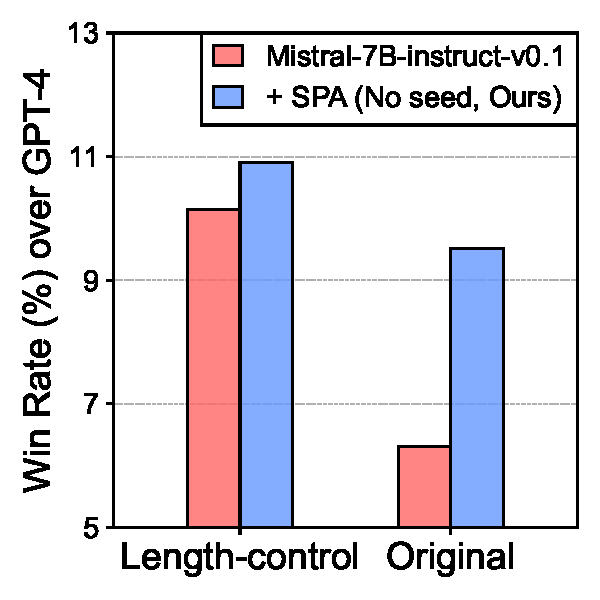
\includegraphics[width=40mm]{figure/raw_files/spa_fig4.pdf}
        \caption{\textbf{无种子数据的提升。} 在 AlpacaEval 2.0 上的评估结果,使用 Mistral-7B-instruct-v0.1 进行实验,并且 SPA 不使用任何种子偏好数据。}
	% \vspace{-0.2cm}
 \label{fig:res_no_seed}
	% }
\end{figure}

\begin{figure}
    \centering
	{
	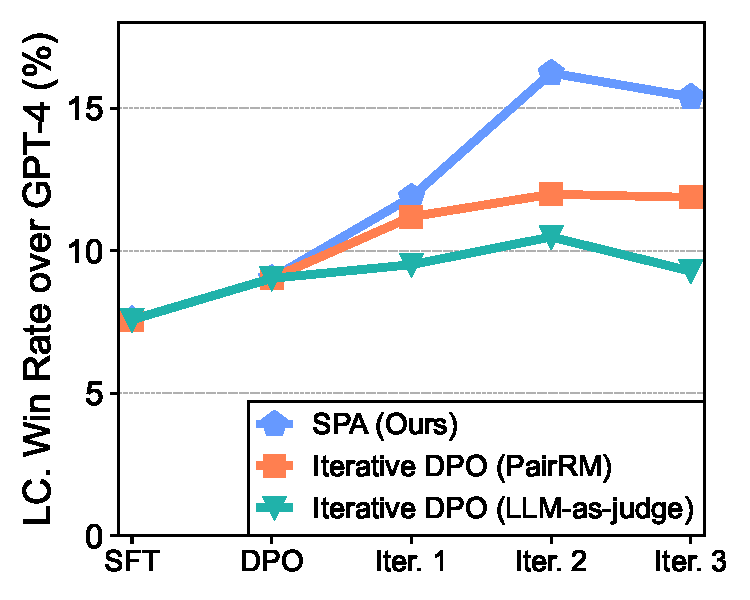
\includegraphics[width=55mm]{figure/raw_files/spa_fig3.pdf}
	\vspace{-0.2cm}
    \caption{\textbf{迭代过程中的提升。} 由 AlpacaEval 2.0 计算的长度控制(LC.)胜率(\%)在 SPA 训练下持续提升,并优于其他基线方法。}\label{fig:res_iteration}
	}
\end{figure}

\begin{table}[t]
    \centering
    \caption{\textbf{不同数量的种子数据。} 在 AlpacaEval 2.0 上,对使用不同数量的种子真实偏好标签训练的 Mistral-7B-v0.1 进行评估,比较 DPO 和 SPA 的表现。}\begin{tabular}{l|cccc}
      \toprule
      & \multicolumn{4}{c}{Used Ground-truth Preference Data} \\
      \cmidrule(lr){2-5}
    Methods  & 0.8\% & 1.7\% & 3.3\% & 10\% \\  \midrule
    DPO: LC Win Rate (\%) & 7.85 & 7.68 & 9.03 & 11.37   \\
    DPO: Win Rate (\%) & 5.53 & 5.49 & 7.68  & 9.32 \\\midrule
    SPA: LC Win Rate (\%) & 10.36 & 12.36 & 16.23 & 18.52  \\
    SPA: Win Rate (\%) & 11.34 & 13.72 & 19.94 & 23.79   \\ 
    \bottomrule
    \end{tabular}
    \label{tab:diff_N_seeds}
\end{table}

\textbf{不同数量种子数据的泛化能力} 
在之前的实验中,我们假设初始仅有少量的人类偏好数据,例如 UltraFeedback 数据集的 3.3\%。
然而,SPA 的有效性并不依赖于种子偏好数据集的规模,我们通过额外的实验对此进行了验证。
首先,我们通过改变种子真实偏好数据的比例来进行实验。
具体而言,为了在每次迭代中使用固定的输入提示数据集,我们在实验中考虑了以下数据比例:[0.8\%、1.7\%、10\%]。
表 \ref{tab:diff_N_seeds} 显示了在 Mistral-7B-v0.1 上进行 2 轮 SPA 训练后的 AlpacaEval 2.0 评测结果,其中也包括使用 3.3\% 种子偏好数据的原始实验。
从结果可以观察到,DPO 和 SPA 的对齐性能随着种子数据的增加而提升,且 SPA 始终优于 DPO,这表明 SPA 在不同种子偏好数据规模下均具有较强的鲁棒性。

此外,我们进一步评估了 SPA 在\textit{无种子偏好数据}情况下的可行性。
具体而言,我们希望回答一个问题:LLM 是否能够利用其在先前训练(如预训练或监督指令微调(SFT))过程中学习到的人类相关知识,在不同响应之间推导出明确的人类偏好。
在该实验中,我们使用 Mistral-7b-instruct-0.1v \citep{jiang2023mistral} 作为初始模型(\textit{i.e.}, $\pi_0$),并使用 Mistral-7b-0.1v-base 作为参考模型(\textit{i.e.}, $\pi_{\text{init}}$)(关于初始设置,请参见第 \ref{sec:method} 节)。
该设置允许我们验证,即使在没有种子偏好数据的情况下,当模型经过充分的迭代数据扩展和自我精调学习后,我们的方法仍然可以有效运行。
如图 \ref{fig:res_no_seed} 所示,胜率从 6.31\% 提升至 9.79\%,长度控制胜率从 10.14\% 提升至 11.59\%。
这一结果表明,即使没有种子数据,SPA 仍然可以利用 LLM 内部信息来对齐人类偏好。

\begin{table}[t]
    \centering
    \caption{\textbf{不同的初始种子。} 在 AlpacaEval 2.0 上,针对不同初始种子偏好数据采样,对 Mistral-7B-v0.1 的不同变体进行评估。}
    \resizebox{\textwidth}{!}{
    \begin{tabular}{l|ccc|cc}
    \toprule 
    {Methods} & {1st Seed Data} & {2nd Seed Data} & {3rd Seed Data} & {Average} & {Variance} \\  
    \midrule
    {DPO: LC Win Rate (\%)} & 9.03 & 8.74 & 9.54 & 9.10 & 0.16 \\ 
    {DPO: Win Rate (\%)} & 7.68 & 7.17  & 7.59 & 7.48 &  0.07 \\ \midrule
    {SPA (Ours): LC Win Rate (\%)} & 16.23 & 13.77 &16.38 & 15.46 & 2.10 \\ 
    {SPA (Ours): Win Rate (\%)} & 19.94 & 20.06 &19.74 & 19.91 & 0.03 \\
    \bottomrule
    \end{tabular}
    }
    \label{tab:variance_seeds}
\end{table}

\textbf{不同初始种子数据集的方差} 
此外,我们进行实验来检验 SPA 对初始种子偏好数据集的敏感性,方法是使用不同的随机采样进行变化。
在 SPA 训练 2 轮后的结果如表 \ref{tab:variance_seeds} 所示。
可以观察到,无论种子数据如何选择,SPA 始终能够提升对齐性能,并且不同种子数据之间的方差并不显著,特别是在标准胜率的情况下。
尽管在长度控制(LC)胜率方面,我们的方法表现出相对较高的方差,但其最低置信区间值(13.36\%)仍然明显高于最强基线模型(11.98\%),
这进一步验证了我们方法的有效性。

\textbf{兼容不同模型} 
接下来,为了验证我们框架在不同 LLM 上的兼容性,我们使用了三种不同的 LLM 进行实验:Phi-2-2.7B \citep{li2023textbooks}、LLaMA3-8B \citep{dubey2024llama} 和 Phi-3-14B。
具体而言,我们基于这些模型的监督微调版本进行实验;对于 Phi-2,我们使用了在 UltraChat 数据集上微调的模型。
\footnote{\url{lole25/phi-2-sft-ultrachat-full}} 
对于 LLaMA-3\footnote{\url{https://huggingface.co/meta-llama/Meta-Llama-3-8B-Instruct}} 
和 Phi-3\footnote{\url{https://huggingface.co/microsoft/Phi-3-medium-4k-instruct}},
由于没有在 UltraChat 数据集上微调的版本,我们使用了它们的通用微调版本。
这些实验的大多数设置与之前的实验保持一致,部分略有调整的实验设置详见附录b.3。% \ref{app:b.3}。
如表 \ref{tab:phi} 所示,实验结果表明,将 SPA 应用于不同的 LLM,能够稳定提升其性能。
例如,在 Phi-2 的实验中,相比 DPO,胜率从 5.67\% 提升至 9.43\%,长度控制胜率从 7.02\% 提升至 9.1\%。
这些结果表明,SPA 的有效性不仅限于特定的 LLM,而是能够在不同的 LLM 上推广并获得稳定的性能提升。

\begin{table}[t]
    \centering
    \caption{\textbf{不同大模型的兼容性。} 在 AlpacaEval 2.0 上,使用不同训练方法(SFT、DPO 和 SPA)对各种大模型(Phi-2-2.7B、LLaMA-3-8B 和 Phi-3-14B)进行评估。最佳分数以 \textbf{加粗} 标出。}
    \resizebox{\textwidth}{!}{
    \begin{tabular}{lc|cc|cc|cc}
    \toprule 
     & & \multicolumn{2}{c|}{\textbf{Phi-2-2.7B}} & \multicolumn{2}{c|}{\textbf{LLaMA-3-8B-Instruct}} & \multicolumn{2}{c}{\textbf{Phi-3-14B-Instruct}} \\
    \cmidrule(lr){3-4} \cmidrule(lr){5-6} \cmidrule(lr){7-8}
    Methods & \begin{tabular}{@{}c@{}} Gold \\ Label (\%)\end{tabular}& \begin{tabular}{@{}c@{}}Len-control. \\ Win Rate (\%)\end{tabular} & \begin{tabular}{@{}c@{}}Win Rate \\ vs. GPT-4 (\%)\end{tabular} & \begin{tabular}{@{}c@{}}Len-control. \\ Win Rate (\%)\end{tabular} & \begin{tabular}{@{}c@{}}Win Rate \\ vs. GPT-4 (\%)\end{tabular} & \begin{tabular}{@{}c@{}}Len-control. \\ Win Rate (\%)\end{tabular} & \begin{tabular}{@{}c@{}}Win Rate \\ vs. GPT-4 (\%)\end{tabular} \\ \midrule
    SFT & - & 5.88 & 3.78 & 21.40 & 21.71 & 26.51 & 21.41  \\
    DPO & 3.3 & 7.02 & 5.67 & 24.17 & 25.39 & 27.70 & 22.12   \\
    SPA (Ours) & 3.3 & \textbf{9.10}  & \textbf{9.43} & \textbf{25.03}  & \textbf{34.84} & \textbf{28.77}  & \textbf{24.14}     \\ 
    \bottomrule
    \end{tabular}
    } 
    \label{tab:phi}
\end{table}

\begin{table}[t]
    \centering
    \caption{\textbf{消融实验。} 在 AlpacaEval 2.0 上,使用不同 SPA 方法配置下的迭代训练模型(从 SFT 开始)进行评估。DE、SR 和 DND 分别是数据扩展、自我优化和去耦噪声检测的缩写。最佳分数以 \textbf{加粗} 标出。}
    \resizebox{0.8\textwidth}{!}{
    \begin{tabular}{l|ccc|cc}
      \toprule
      & & & & \multicolumn{2}{c}{\textbf{AlpacaEval 2.0}}  \\
    \cmidrule(lr){5-6} 
      {Methods} & DE & SR & DND & \begin{tabular}{@{}c@{}}Len-control. \\ Win Rate (\%)\end{tabular} & \begin{tabular}{@{}c@{}}Win Rate \\ vs. GPT-4 (\%)\end{tabular} \\  \midrule
    SFT & - & - & - & 7.58 & 4.72   \\
    DPO & - & - & - & 9.03 & 7.68  \\ \midrule
        & O & X & X  & 14.41  & 19.91 \\
    SPA (Ours) & O & O & X  & 14.7 & 19.94 \\ 
      & O & O & O  & \textbf{15.39} & \textbf{21.13}  \\ 
    \bottomrule
    \end{tabular}
    }
    \label{tab:ablation}
\end{table}

\begin{table}[t]
    \centering
    \caption{\textbf{附加分析。} 在 AlpacaEval 2.0 上,使用不同判断方法对从 SPA 第一次迭代结果模型进行微调的模型进行评估的结果。}
    \resizebox{0.8\textwidth}{!}{ % 让表格缩放到页面宽度
    \begin{tabular}{l|cc}
    \toprule
     & \multicolumn{2}{c}{\textbf{AlpacaEval 2.0}} \\
    \cmidrule(lr){2-3} 
    Models & \begin{tabular}{@{}c@{}}Len-control. \\ Win Rate (\%)\end{tabular} & \begin{tabular}{@{}c@{}}Win Rate \\ vs. GPT-4 (\%)\end{tabular} \\ \midrule
    SPA after iteration 1  & 10.57 & 11.89  \\   \midrule
    Eq. \ref{eq:our_pref} with initial SFT model (Ours) & 15.08 & 19.56   \\ 
    Eq. \ref{eq:our_pref} with previous model & 13.73  & 17.66   \\ 
    Judgment with PairRM & 13.57  & 13.72   \\
    Judgment without reference model & 12.83  & 12.35  \\
    \bottomrule
    \end{tabular}
    } % 结束 \resizebox
    \label{tab:add_analyses}
\end{table}

\textbf{消融研究} 
为了评估自我优化(self-refinement)组件的影响,我们进行了消融实验,分别移除自我优化(SR)和解耦噪声检测(DND),并在此基础上对现有框架进行实验。
实验结果如表 \ref{tab:ablation} 所示。
当仅使用自我优化但不包含解耦噪声检测(参见公式 \ref{eq:self_refine_combined})时,我们观察到性能略有提升,对 GPT-4 的胜率从 19.91\% 轻微上升至 19.94\%,长度控制胜率从 14.41\% 提升至 14.7\%。
然而,当在自我优化过程中引入了解耦噪声检测(参见公式 \ref{eq:noise_realign})后,性能得到显著提升,胜率从 19.91\% 提升至 21.13\%,长度控制胜率从 14.41\% 提升至 15.39\%。
此外,这些结果表明,自我优化组件是提升性能的关键因素,有助于提高胜率并改善长度控制。

\textbf{关于偏好判断方法的额外分析}  
在表 \ref{tab:add_analyses} 中,我们进一步分析了偏好判断过程中参考模型的影响(参见公式 \ref{eq:our_pref})。
该分析针对从第 1 轮到第 2 轮的训练过程进行,此时观测到了最显著的性能变化(即,我们从第 1 轮的模型开始微调)。
为了单独比较不同判断方法的影响,我们遵循表 \ref{tab:judgments} 的设置,并排除了自我优化组件的影响。
然后,我们设计了三种实验方案:(1)使用上一轮的策略模型作为参考模型,(2)不使用任何参考模型进行判断,(3)使用 PairRM 进行判断。

实验结果如表 \ref{tab:add_analyses} 所示。
结果表明,在 SPA 方法中,使用 SFT 模型作为参考模型进行偏好判断可以获得最高的性能提升。
具体而言,使用上一轮的模型作为参考模型时,性能较低,且长度控制胜率下降幅度(15.08\% vs 13.73\%)大于胜率下降幅度(19.56\% vs 17.66\%)。
尽管如此,该方法仍然优于使用 PairRM 进行判断。

这些结果可能表明,在训练过程中使用 LLM 本身进行偏好判断比使用外部模型更为重要,因为这样可以减少分布不匹配带来的影响。
然而,在不使用参考模型的情况下(即,仅使用当前模型的似然值),其性能提升幅度是所有方法中最低的。
这些结果进一步强调了选择合适的判断方法和参考模型对整体性能的显著影响。

\section{结论}
在本文中,我们提出了 SPA,一种可以通过最少的人类标注偏好数据高效提升大模型对齐度的方法。
我们的主要贡献包括:开发了一种有效的数据扩展方法,结合了直接偏好判断方法,以及一种自我优化(潜在的)噪声偏好的偏好学习算法。
我们通过在各种设置下微调近期的大模型,并在常用基准测试 AlpacaEval 2.0 和 MT-Bench 上进行评估,展示了 SPA 的有效性,并观察到显著的提升。
我们期待 SPA 在未来的研究和实际应用中做出重要贡献,特别是在难以收集人类标注偏好的情况下。有关局限性和社会影响的讨论,请参见附录A。


\begingroup
    \linespreadsingle{} 
    \printbibliography[title={外文翻译参考文献}]
\endgroup
